%\chapter{M3DA datasets description}
%\label{app:m3da_datasets}
%
%
%Below we provide an extended description of datasets used in M3DA benchmark, download and usage examples are available in the published repository\footnote{\href{https://github.com/BorisShirokikh/M3DA}{https://github.com/BorisShirokikh/M3DA}}. Example 2D slices from every dataset for visual comparison between domains are given in Figure~\ref{fig:contours}. Summary of licenses and data access is given in Table~\ref{tab:supp_datasets}.
%
%\begin{table}[h]
	\centering
	\caption{Datasets licenses and independent source links.}
	
	\resizebox{\linewidth}{!}{%
		\begin{tabular}{@{}lcc@{}}
			\toprule
			\textbf{Dataset} & license & link to dataset \\
			\midrule
			BraTS \cite{brats} & CC BY 4.0  & \href{https://www.cancerimagingarchive.net/analysis-result/rsna-asnr-miccai-brats-2021/}{https://www.cancerimagingarchive.net/analysis-result/rsna-asnr-miccai-brats-2021/} \\
			
			CC359 \cite{cc359} & CC BY-ND 4.0 & \href{https://www.ccdataset.com/download}{https://www.ccdataset.com/download}  \\
			
			AMOS \cite{amos} & CC BY 4.0 & \href{https://zenodo.org/records/7262581}{https://zenodo.org/records/7262581} \\
			
			AMOS LDCT & CC BY 4.0 & \href{https://zenodo.org/records/13373720}{https://zenodo.org/records/13373720} \\
			
			LIDC \cite{lidc} & CC BY 3.0 & \href{https://www.cancerimagingarchive.net/collection/lidc-idri/}{https://www.cancerimagingarchive.net/collection/lidc-idri/}\\
			
			\bottomrule
		\end{tabular}
	}
	\label{tab:supp_datasets}
\end{table}
%
%
%\section{AMOS}
%
%The AMOS dataset \cite{amos} contains 500 CT and 100 MRI abdominal scans with the multi-organ segmentation task: liver, stomach, spleen, left and right kidneys, bladder, aorta, pancreas, inferior vena cava, duodenum, prostate/uterus, gallbladder, esophagus, left and right adrenals. As a largest available dataset for inter-modality segmentation, we employed it in MR$\ra$CT and CT$\ra$MR domain shift setups. 
%
%We used all 60 labeled MRIs as the \textit{source} set in MR$\ra$CT setup and the \textit{target test} set in CT$\ra$MR. Then, 200 unlabeled CTs and 40 unlabeled MRIs were used as the \textit{target train} sets for adaptation purposes in the MR$\ra$CT and CT$\ra$MR setups, respectively. The remaining 300 labeled CTs were evenly split in two groups: the first is a source set in CT$\ra$MR, and the second is a target test set in MR$\ra$CT.
%
%Furthermore, we used AMOS CT images to create one of the most clinically relevant domain shift setups -- difference in the radiation dose during scanning. 
%% In CT$\ra$LDCT, we employed the first group of 150 labeled CTs as a source set, 200 unlabeled CTs as a target train set, and the second group of 150 labeled CTs as a target test set. 
%For the LDCT domain, we simulated low radiation dose using the algorithm provided in \cite{ldct}, simulated data are available at \href{https://zenodo.org/records/13373720}{https://zenodo.org/records/13373720}.
%
%
%\section{BraTS}
%
%BraTS \cite{brats} is comprised of 2000 brain MRI cases, each consisting of four sequences: T1, T1c, T2, FLAIR, with a glioblastoma segmentation classes (3 foreground classes and background).  We only used 1251 cases with publicly available annotations and T1, T1c MRI sequences for T1 CE$\ra$T1 shift. Since sequences of the same case provide information about the same subject, we ensured source-target splits so that every case falls into exactly one fold and split cases with 50:25:25 ratio into source, target train, and target test folds.
%
%
%\section{CC359}
%
%The CC359 dataset \cite{cc359} contains 359 brain MR T1 images from three scanners, namely, GE, Philips (PH), and Siemens (SM), obtained using two magnetic field strength values, $1.5$ and $3.0$T. The dataset can be split into six domains defined by two different field strengths $\times$ three vendors, each with approximately 60 images, so it yields 30 possible domain adaptation pairs. 
%
%CC359 also offers three tasks: brain, hippocampus, and white matter, gray matter, and cerebrospinal fluid (WMGMCSF) segmentation. We ommited hippocampus segmentation task from the benchmark, because our preliminary experiments showed it is not significantly affected by domain shifts, the relative performance drop is less than $2\%$ in every domain pair; see Table~\ref{tab:hippo}. We also omitted the brain segmentation task for the same reason, see results in \cite{shirokikh2020first}.
%
%

\begin{table}[h]
	\centering
	\caption{Baseline and oracle results on the CC359 WMGMSCF segmentation task.}
	\label{tab:wmgmcsf}
	
	% \resizebox{\columnwidth}{!}{%
		\begin{tabular}{|c|l||c|c|c|c|c|c|}
			
			\hline
			\multicolumn{2}{|l||}{\multirow{2}{*}{}}  & \multicolumn{6}{c|}{Target domains}\\ 
			\cline{3-8}
			\multicolumn{2}{|l||}{} & GE1.5 & PH1.5 & SM1.5 & GE3.0 & PH3.0 & SM3.0\\ 
			\hline
			\hline
			
			% \clrtb
			
			\multirow{6}{*}{{\rotatebox[origin=c]{90}{Source domains}}}
			& GE 1.5 & 95.8 & 82.1 & 90.8 & 82.1 & 92.6 & 80.8 \\
			\cline{2-8}
			
			& PH 1.5 & 80.1 & 92.7 & 90.8 & 93.4 & \textbf{74.1} & 90.1 \\
			\cline{2-8}
			
			& SM 1.5 & 89.7 & 85.3 & 95.6 & 86.2 & 86.2 & 84.5 \\
			\cline{2-8}
			
			& GE 3.0 & 76.6 & 89.9 & 90.3 & 95.9 & 72.0 & 91.4 \\
			\cline{2-8}
			
			& PH 3.0 & 90.6 & 74.7 & 86.0 & 75.4 & 95.4 & \textbf{76.6} \\
			\cline{2-8}
			
			& SM 3.0 & \textbf{56.0} & 88.6 & 84.9 & 92.4 & 68.4 & 95.7 \\
			\hline
			
		\end{tabular}%}
\end{table}


\begin{table}[h]
	\centering
	\caption{Baseline and oracle results on the CC359 hippocampus segmentation task.}
	\label{tab:hippo}
			
	%\resizebox{\columnwidth}{!}{%
		\begin{tabular}{|c|l||c|c|c|c|c|c|} 
			\hline
			\multicolumn{2}{|l||}{\multirow{2}{*}{}}  & \multicolumn{6}{c|}{Target domains}\\ 
			\cline{3-8}
			\multicolumn{2}{|l||}{} & GE1.5 & PH1.5 & SM1.5 & GE3.0 & PH3.0 & SM3.0 \\ 
			\hline
			\hline
			
			% \clrtb
			
			\multirow{6}{*}{{\rotatebox[origin=c]{90}{Source domains}}}
			& GE 1.5 & 92.3 & 86.7 & 88.7 & 87.8 & 91.2 & 91.2 \\
			\cline{2-8}
			
			& PH 1.5 & 91.3 & 86.9 & 87.7 & 87.7 & 89.7 & 89.9 \\
			\cline{2-8}
			
			& SM 1.5 & 91.7 & 86.6 & 89.3 & 88.2 & 90.9 & 90.8 \\
			\cline{2-8}
			
			& GE 3.0 & 91.4 & 86.4 & 88.0 & 89.1 & 90.5 & 91.3 \\
			\cline{2-8}
			
			& PH 3.0 & 91.5 & 86.5 & 88.3 & 87.7 & 92.0 & 91.0 \\
			\cline{2-8}
			
			& SM 3.0 & 90.8 & 86.5 & 87.8 & 88.0 & 90.6 & 92.1 \\
			\hline
			
	\end{tabular}%}
\end{table}

%
%Therefore, we focus only on the WMGMCSF segmentation task in CC359: white matter, gray matter and cerebral spinal fluid segmentation classes and background. From 30 possible domain pairs, we selected three with the maximum performance drop, highlighted in \textbf{bold},  Table~\ref{tab:wmgmcsf}): changing field strength with a fixed scanner PH 1.5T $\ra$ PH 3.0T (drop from 95.4 to 74.1 Dice score), changing scanner with the fixed field strength PH 3.0T $\ra$ SM 3.0T (drop from 95.7 to 76.6), and changing both parameters SM 3.0T $\ra$ GE 1.5T (drop from 95.8 to 56.0). We denote them as T1 F, T1 Sc, and T1 Mix, respectively.
%
%
%\section{LIDC}
%
%LIDC \cite{lidc} is a multi-center collection of diagnostic and lung cancer screening thoracic CT scans with annotated lesions. It includes 1308 studies (of which 1018 include CT studies) from 1010 patients. Lung's nodules is one of the few clinical applications where both CE CT and CT are used, first for the initial scan, and second for the follow-ups \cite{purysko2016does}. We used LIDC for CE CT $\ra$ CT domain shift, we split data into three roughly equal groups, ommiting scans with empty masks: contrast enhanced CT (source domain) $X^s$, CT without contrast enhancement $X^t_{tr}$ (training part, target domain), and CT without contrast enhancement  $X^t_{ts}$ (test part, target domain). $X^t_{tr}$ and $X^t_{ts}$ were stratified by the number of lesions.
%
%
%\chapter{M3DA methods description}
%\label{app:m3da_methods}
%
%As mentioned above, we used an nnU-Net \cite{nnunet} backbone as segmentation network architecture in all methods. We preserved most of the nnU-Net training pipeline except for several methodological changes, which allow us to evaluate DA methods, such as AdaBN and InstanceNorm, separately and run the ablation studies. These changes along with the other training hyper-parameters are summarized in Table~\ref{tab:hyper}.
%
%Firstly, we replaced the default InstanceNorm with BatchNorm layers and removed test-time augmentation, so we can compare different normalizations and adaptive normalizations (AdaBN) and assess the unhindered impact of DA methods. Secondly, we reduced the patch size and number of the network features, so all experiments fit in a single 16 GB NVIDIA Tesla V100 and our benchmark remains economical. We set the number of epochs to 600 in all experiments, so that any method could complete its training in three days. All experiments were conducted on the Zhores supercomputer~\cite{zacharov2019zhores}.
%
%

\begin{table}[h]
	\centering
	\caption{Hyper-parameters.}
	\label{tab:hyper}
	%\resizebox{\linewidth}{!}{
		\begin{tabular}{lcc}
			\toprule 
			\textbf{hyper-parameter} & \textbf{nnUNet} & \textbf{U-Net (ours)}  \\ 
			\midrule
			architecture & auto & auto \\
			base features & 32 & 24 \\
			normalization & instance (IN) & batch (BN) \\
			batch size & 2 & 2 \\
			patch size & (160, 192, 64) & (160, 160, 64) \\
			epochs & 600 & 600 \\
			batches per epoch & 250 & 250 \\
			loss & Dice Loss + CE & Dice Loss + CE \\
			% loss masking based on intensity & \cmark & \xmark \\
			oversampling rate & 0.66 & 0.75 \\
			optimizer & SGD & SGD \\
			momentum & 0.99 & 0.99 \\
			weight decay & $3 \times 10^{-5}$  & $3 \times 10^{-5}$ \\
			initial learning rate & $10^{-2}$ & $10^{-2}$ \\
			learning rate schedule & poly decay & poly decay \\
			learning rate decay power & 0.9 & 0.9 \\
			test-time augmentation & \cmark & \xmark \\
			\bottomrule
	\end{tabular}%}
\end{table}

%
%Below, we provide DA methods implementation details:
%
%\paragraph{Histogram matching} uses the baseline training pipeline, except all image intensity histograms are equalized to an average histogram computed over the train set. 
%
%\paragraph{Gamma augmentation} also uses the baseline training pipeline, and we perform gamma correction with randomly selected $\gamma \sim U[0.5, 2]$ on every input image.
%
%\paragraph{nnAugm} similarly supplements the same baseline training with the original set of nnUNet \cite{nnunet} augmentations.
%
%\paragraph{InstanceNorm} substitutes BN layers, while the training pipeline remains the same as in baseline.
%
%\paragraph{Adaptive BN} performs additional 1000 inference steps with batch size 4 over the baseline, updating the running statistics of BN layers on target training data.
%
%\paragraph{Self-ensembling} design and all parameters are reproduced from \cite{se_medim} with our architecture.
%
%\paragraph{MinEnt} adds a predictions entropy minimization criterion on target images. So we extended our training pipeline with the second step using target train images, and added entropy loss with the recommended in \cite{entropy} weight $\lambda = 0.001$.
%
%\paragraph{DANN} introduces an auxiliary network called discriminator. Similar to recent studies \cite{entropy}, we used DCGAN~\cite{dcgan} discriminator architecture, replacing 2D convolutions with 3D ones. The losses weighting parameter is taken from \cite{dann_medim}, e.g., $\alpha = 0.01$.
%
%\paragraph{CycleGAN 2D} is fully reused from the original study \cite{cyclegan}. We trained a standalone CycleGAN 2D to map between source and target train images, where we sample axial slices from our volumetric images and rescale them into 256 $\times$ 256 gray scale images. Before predicting with the baseline segmentation model, we applied one of the generators to target test images (slice-by-slice) to transform them into fake source ones.
%
%\paragraph{CycleGAN 3D} is fully reused from the original study \cite{cyclegan3d}. We trained a standalone CycleGAN 3D to map between source and target train images, where we sample patches of size (128, 128, 96) from our volumetric images. Before predicting with the baseline segmentation model, we applied one of the generators to target test images (via overlapping grid) to transform them into fake source ones.
%
%\paragraph{GIN} is fully reused from \cite{gin} with the implementation based on the nnU-Net framework.
%
%\paragraph{MIND} is fully reused from \cite{dg_tta} with the implementation based on the nnUNet framework.\\
%
%
%All experiments are available at \href{https://github.com/BorisShirokikh/M3DA-exp}{github.com/BorisShirokikh/M3DA-exp}.


%\chapter{Evidence of Industrial Application}
%\label{app:m3da_datasets}
\chapter{Certificate of Registration}
\label{app:reg}

\begin{center}
	%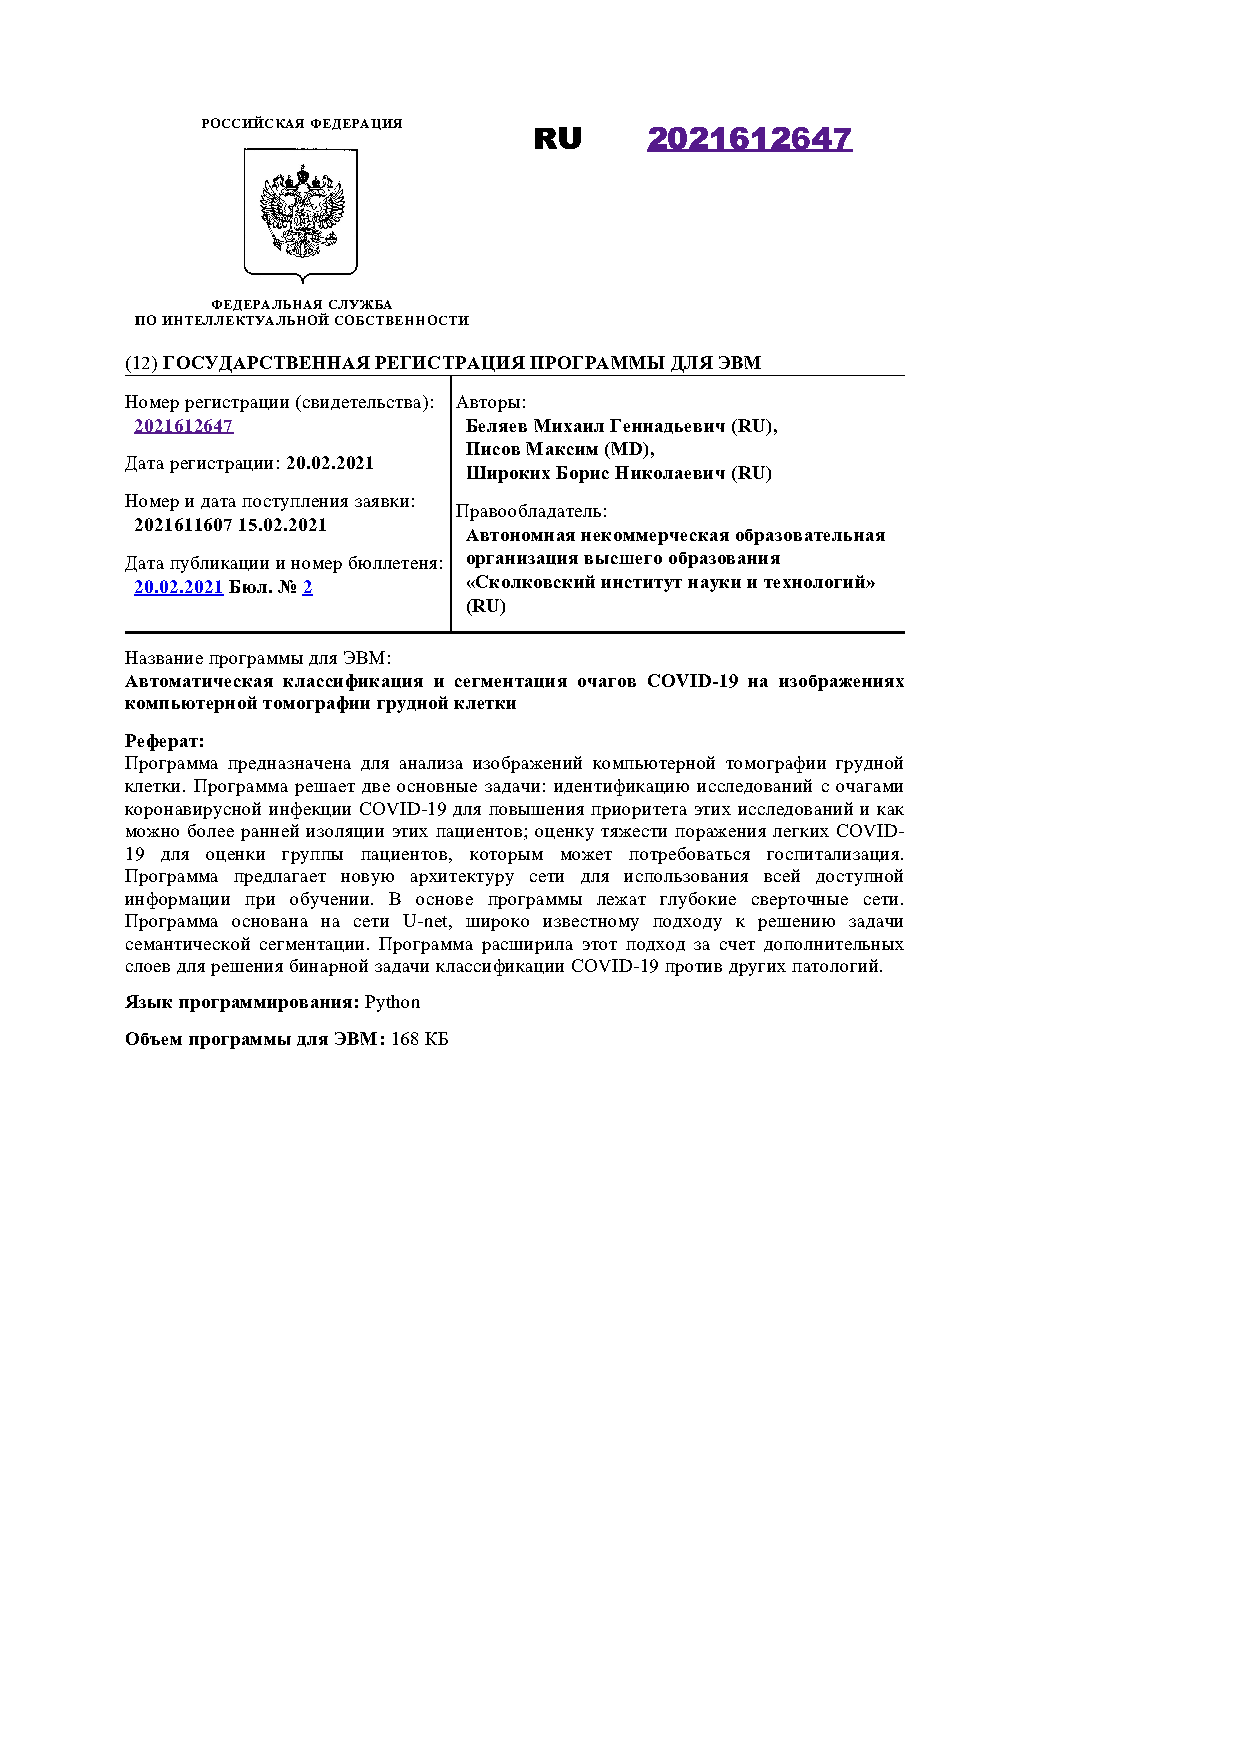
\includegraphics[width=\textwidth]{Dissertation/Figures/6_appendix/output.pdf}
	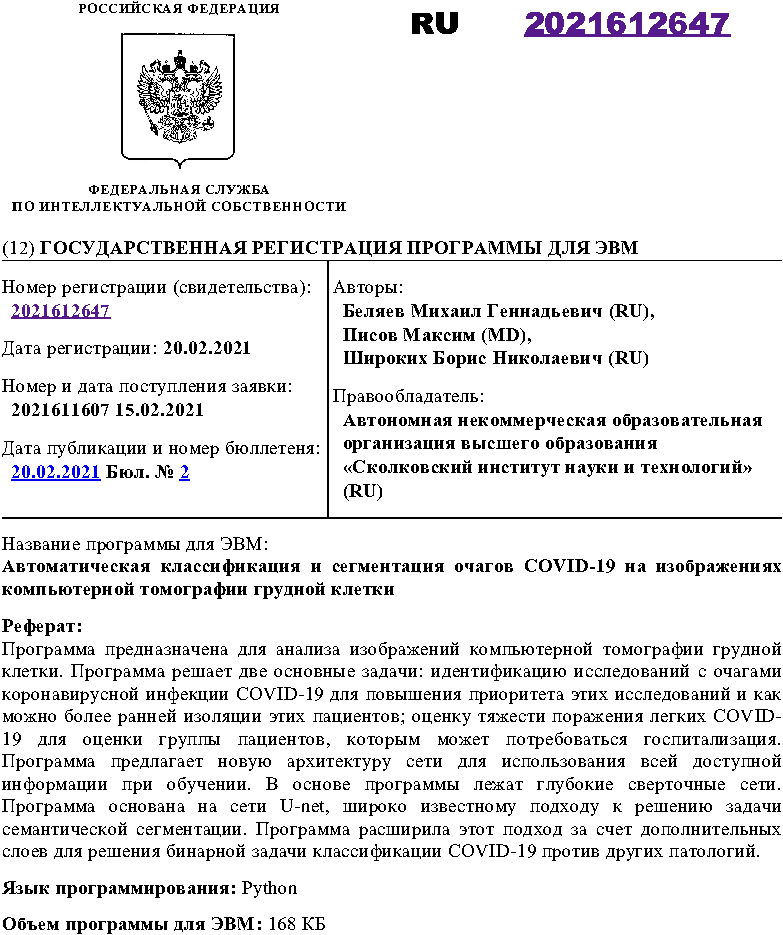
\includegraphics[width=0.95\textwidth]{Dissertation/Figures/6_appendix/output_crop.pdf}
\end{center}

